\section{Experimental System}

Two separate experimental systems were used when testing and gathering results for localization and motion planning. The first of these is the physical robot, HARLIE, which will be described in further detail in \autoref{subsec:harlie_setup}. The second experimental system is a simulation environment which will be described in detail in \autoref{subsec:simulation_setup}.

\subsection{HARLIE}\label{subsec:harlie_setup}

\begin{figure}

\centering
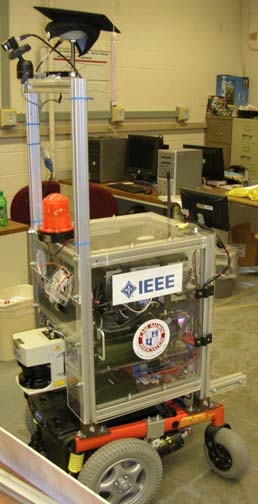
\includegraphics{images/harlie}
\caption{HARLIE, the robot used for experimental testing \label{fig:harlie}}

\end{figure}

The physical robot used for these experiments was HARLIE (see \autoref{fig:harlie}). HARLIE is a fully autonomous robot built on top of a wheelchair base donated by the Invacare Corportation. The robot is powered via a pair of car batteries in series, providing a nominal twenty-four volts to the system. The wheelchair base has two electric motors powering the two drive wheels; with one motor per wheel, HARLIE is able to vary the velocity of each drive wheel independently. Because of this independent velocity control, HARLIE can move forwards and backwards, both straight and in arcs, as well as spin in place. This drive setup is known as ``differential drive'' and is one of the most common drive setups used in mobile robotics \autocite{Lav06}.

On top of this differential drive base, HARLIE is equipped with numerous sensors and computing systems.

\subsection{Simulation}\label{subsec:simulation_setup}

Gazebo simulation
